\chapter{Competition Regulations}

\section{Definition of Each Category}

\begin{enumerate}
\item TANDING (Sparring Match) category is the category of Pencak Silat competition that confronts 2 (two) Pesilat from different teams. Both of them confront each other by using the elements of self-defence and attacking such as defending/avoiding/hitting/attacking the target and dropping the opponent; the use of competition techniques and tactics, stamina and endurance, and fighting spirit, using the principles and using the richness of movement of techniques.

\url{https://youtu.be/Sy1wCmHILnA}


TUNGGAL (Solo Performance) is the category of Pencak Silat competition performed by one Pesilat that performs his skill in Jurus Tunggal Baku (Solo Compulsory Movement), accurately and firmly, complete soulfully with empty hands and with weapons according to rules and regulations apply for Tunggal category.

\url{https://youtu.be/_fcd-27kMhE}

\item GANDA (Choreographed Pair Performance) is the category of Pencak Silat competition which features two Pesilat of the same team performs choreographed technical skills rich of attacking – defensive movement of Pencak Silat. The movement of the attacking-defensive movement is performed with a well planned, effective, aesthetical, powerful and in an orderly series, with empty hands or with weapon according to rules and regulations apply for Ganda category.

\url{https://youtu.be/eUsunr0dTKk}

\item REGU (Synchronized Team Performance) category is the category of Pencak Silat competition which is performed by 3 (three) Pesilat from the same team portraying their skills in a compulsory movements correctly, accurately, firmly, complete with expression, synchronize and compact with empty hands according to rules and regulations apply for Regu category 

\url{https://youtu.be/Q6JSm8Mcd4w}

\end{enumerate}



\section{Classification of Competitions and Regulation of Age, Gender and Weight}


\begin{legal}
\item The top-level classifications of Pencak Silat competitions according to age, gender and weight for all categories consist of:
    \begin{legal}
    \item USSSA / USA Youth
        \begin{legal}
        \item Competition of USA-JUNIOR-I for Male and Female aged 10 to 11 years.
        \item Competition of USA-JUNIOR-II for Male and Female aged 12 to 14 years.
        \item Competition of USA-JUNIOR-III for Male and Female aged 15 to 16 years.
        \end{legal}
    \item PERSILAT / International Youth
        \begin{legal}
        \item Competition of PRE-TEEN for Male and Female aged over 10 to 12 years.
        \item Competition of PRE-JUNIOR for Male and Female aged over 12 to 14 years.
        \item Competition of JUNIOR for Male and Female aged over 14 to 17 years
        \end{legal}
    \item Adult
        \begin{legal}
        \item Competition of SENIOR for Male and Female aged over 17 to 35 years.
        \item Competition of MASTER-I for Male and Female aged over 35 to 45 years
        \item Competition of MASTER-II for Male and Female aged over 45 years
        \end{legal}
    \end{legal}

\item Confirmation of the age and citizenship (refer to annex) of a Pesilat participating in Competition is proved by a birth certificate, diploma, original passport or certified true Copy documents.

\item The age of Pesilat must confirm with the classification of age of the participants on the first day of the competition (regardless of any competition category).

\item The classification of classes according to body weight is valid only for TANDING category which is performed by weighing in.

    \begin{legal}
    \item No tolerance of body weight.
    \item The weigh-in is carried out 15 (fifteen) minutes before the start of the match in one Championship according to the schedule of the competition.
During the weigh-in the Pesilat (contestant) must wear a Pencak Silat unform using for competition, dry, without sash, without groin guard or any joint guards.
    \item A Pesilat (contestant) whose weight fails to meet his/her class requirement during weigh-in will be disqualified from the competition.  
The weigh-in is only carried out once and must be witnessed by officials from both teams and a referee-jury on duty. 
    \item It is mandatory for the weigh-in officials and officials from both teams to sign the weigh-in form which is provided by the Organizing Committee. When one of the team officials failed to endorse the form them weigh-in remains valid.
    \item The weigh-in officials are appointed by the organizing committee.
    \end{legal}

\item Certification of Medical Checkup
    \begin{legal}
    \item Every Pesilat (contestant) should produce a certified medical certificate, i.e. a letter to prove good health issued by authorized doctor or hospital/clinic, 1 month maximum before the first of competition regardless of competition category. 
    \item A Pesilat (contestant) who failed to show the medical certification before weighing in will be disqualified from the competition. 
    \end{legal}
    Organizing committee may recommend a certain doctor/hospital in the hosting country/city where cost is borne by the team of Pesilat. 
\end{legal}


\section{Youth Classifications}

\begin{legal}
\item USSSA / Domestic Youth Classifications

For domestic competition, USSSA has established classifications to align with divisions and levels 
found in other youth sports and martial arts competitions in the United States.  These are referred to as USA JUNIOR I, II and III resepectively.  These three levels are further detailed in~\ref{sec:usa_junior}.

\item PERSILAT / International Youth Classifications

PERSILAT Youth Classes are used in international competition. For consistency with other
    PERSILAT member organizations, the same nomenclature of PRE-TEEN, PRE-JUNIOR, JUNIOR is adopted in this
    technical manual.  These three levels are further detailed in~\ref{sec:pre_teen}--\ref{sec:junior}
\end{legal}


\section{Adult Classifications}

Adult categories and classifications are identical for both USSSA and PERSILAT. The same nomenclature of SENIOR,
MASTER-I and MASTER-II is adopted in this technical manual.  These three levels are further detailed 
    in~\ref{sec:senior}--\ref{sec:master}


\section{Categories and Classes of USA Junior I, II, III}
\label{sec:usa_junior}

Categories and classes of USA Junior I, II and III in USSSA domestic competition:

\begin{legal}
\item Event Categories
    \begin{legal}
    \item Tanding (Sparring Match)
    \item Tunggal (Solo Performance)
    \item Ganda (Choreographed Pair Performance)
    \item Regu (Synchronized Pair Performance)
    \end{legal}
\item Across all event categories USA Youth classes consists of the following division breakdowns:
    \begin{legal}
    \item Age Bracket
        \begin{legal}
        \item USA Junior I: 10 to 11 years of age 
        \item USA Junior II: 12 to 14 years of age 
        \item USA Junior III: 15 to 16 years of age 
        \end{legal}
    \item Gender
        \begin{legal}
        \item Male
        \item Female
        \end{legal}
    \item No weight classes 
    \item Skill levels
        \begin{legal}
        \item Beginner
        \item Intermediate
        \item Advanced
        \end{legal}
    Skill levels is assessed by athlete's Coach and provided at the time of event registration
    \end{legal}


\end{legal}

\section{Categories and Classes of Pre-Teen Competition}
\label{sec:pre_teen}

Categories and classes of Pre-Teen in PERSILAT international competition:

\begin{legal}
\item \strong{Tanding} (Sparring Match) consists of:
    \begin{legal}
    \item Male Tanding (Putra)
        \begin{legal}
        \item Class A 45 kg up to 50 kg
        \item Class B 50 kg up to 55 kg
        \item Class C 55 kg up to 60 kg
        \item Class D 60 kg up to 75 kg
        \item Class E 65 kg up to 70 kg
        \item Class F 70 kg up to 75 kg
        \item Class G 75 kg up to 80 kg
        \item Class H 80 kg up to 80 kg
        \item Class I 85 kg up to 90 kg
        \item Class J 90 kg up to 95 kg
        \item Class Open 85 kg and over
        \end{legal}
    \item Female Tanding
        \begin{legal}
        \item Class A 45 kg up to 50 kg
        \item Class B 50 kg up to 55 kg
        \item Class C 55 kg up to 60 kg
        \item Class D 60 kg up to 75 kg
        \item Class E 65 kg up to 70 kg
        \item Class F 70 kg up to 75 kg
        \item Class Open 65 kg and over
        \end{legal}
    \item \strong{Tunggal} (Solo Performance) consists of:
        \begin{legal}
        \item Tunggal Putra (male solo performance)
        \item Tunggal Putri (female solo performance)
        \end{legal}

    \item \strong{Ganda} (Choreographed Pair Performance) consists of:
        \begin{legal}
        \item Ganda Putra (male choreographed pair performance)
        \item Ganda Putri (female choreographed pair performance)
        \end{legal}

    \item \strong{Regu} (Synchronized Team Performance) consist of:
        \begin{legal}
        \item Regu Putra (male synchronized team performance)
        \item Regu Putri (female synchronized team performance)
        \end{legal}
    \end{legal}


    A Pesilat may participate in any/all Tanding/Tunggal/Ganda/Regu categories as long as he/she 
    meets requirements.

\end{legal}


\section{Categories and Classes of Junior Competition}
\label{sec:junior}

Categories and classes of Junior in PERSILAT international competition:

\begin{legal}
\item \strong{Tanding} (Sparring Match) consists of:
    \begin{legal}
    \item Male Tanding (Putra)
        \begin{legal}
        \item Class A 39 kg up to 43 kg
        \item Class B over 43 kg up to 47 kg 
        \item Class C over 47 kg up to 51 kg
        \item Class D over 51 kg up to 55 kg  
        \item Class E over 55 kg up to 59 kg  
        \item Class F over 59 kg up to 63 kg  
        \item Class G over 63 kg up to 67 kg  
        \item Class H over 67 kg up to 71 kg  
        \item Class I over 71 kg up to 75 kg  
        \item Class J over 75 kg up to 79 kg  
        \item Class K over 79 kg up to 83 kg 
        \item Class L over 83 kg up to 87 kg  
        \item Open Class over 87 kg up to 99 kg
        \end{legal}
    \item Female Tanding (Putri)
        \begin{legal}
        \item Class A 39 kg up to 43 kg
        \item Class B 43 kg up to 47 kg
        \item Class C over 47 kg up to 51 kg
        \item Class D over 51 kg up to 55 kg
        \item Class E over 55 kg up to 59 kg
        \item Class F over 59 kg up to 63 kg
        \item Class G over 63 kg up to 67 kg
        \item Class H over 67 kg up to 71 kg
        \item Class I over 71 kg up to 75 kg
        \item Class J over 75 kg up to 70 kg
        \item Open Class over 79 kg up to 91 kg
        \end{legal}
    \item \strong{Tunggal} (Solo Performance) consists of:
        \begin{legal}
        \item Tunggal Putra (male solo performance)
        \item Tunggal Putri (female solo performance)
        \end{legal}

    \item \strong{Ganda} (Choreographed Pair Performanec) consists of:
        \begin{legal}
        \item Ganda Putra (male choreographed pair performance)
        \item Ganda Putri (female solo performance)
        \end{legal}

    \item \strong{Regu} (Synchronized Team Performance) consist of:
        \begin{legal}
        \item Regu Putra (male team)
        \item Regu Putri (female team)
        \end{legal}
    \end{legal}
\end{legal}

    A Pesilat may participate in any/all Tanding/Tunggal/Ganda/Regu categories as long as he/she 
    meets requirements.


\section{Categories and Classes of Senior Competition}
\label{sec:senior}

Categories of Senior Competition

\begin{legal}
\item \strong{Tanding} (Sparring Match) consists of:
    \begin{legal}
    \item Male Tanding (Putra)
        \begin{legal}
        \item Class A 45kg up to 50kg
        \item Class B over 50kg up to 55kg
        \item Class C over 55kg up to 60kg
        \item Class D over 60kg up to 65kg
        \item Class E over 65kg up to 70kg
        \item Class F over 70kg up to 75kg
        \item Class G over 75kg up to 80kg
        \item Class H over 80kg up to 85kg
        \item Class I over 85kg up to 90kg
        \item Class J over 90kg up to 95kg
        \item Open Class over 85kg
        \end{legal}
    \item Female Tanding (Putri)
        \begin{legal}
        \item Class A 45 kg up to 50 kg
        \item Class B over 50 kg up to 55 kg
        \item Class C over 55 kg up to 60 kg
        \item Class D over 60 kg up to 65 kg
        \item Class E over 65 kg up to 70 kg
        \item Class F over 70 kg up to 75 kg
        \item Open Class over 65 kg
        \end{legal}
    \item \strong{Tunggal} (Solo Performance) consists of:
        \begin{legal}
        \item Tunggal Putra (male solo performance)
        \item Tunggal Putri (female solo performance)
        \end{legal}

    \item \strong{Ganda} (Choreographed Pair Performance) consists of:
        \begin{legal}
        \item Ganda Putra (male choreographed pair performance)
        \item Ganda Putri (female choreographed pair performance) 
        \end{legal}

    \item \strong{Regu} (Synchronized Team Performance) consist of:
        \begin{legal}
        \item Regu Putra (male synchronized team performance)
        \item Regu Putri (female synchronized team performance)
        \end{legal}
    \end{legal}


    A Pesilat may participate in any/all Tanding/Tunggal/Ganda/Regu categories as long as he/she 
    meets requirements.
\end{legal}

\section{Categories and Classes of Master I-II Competition}
\label{sec:master}
Categories of Master Competition

\begin{legal}
\item \strong{Tanding} (Sparring Match) consists of:
    \begin{legal}
    \item Male Tanding (Putra)
        \begin{legal}
            \item Class A 45 kg up to 50 kg
            \item Class B over 50 kg up to 55 kg
            \item Class C over 55 kg up to 60 kg
            \item Class D over 60 kg up to 65 kg
            \item Class E over 65 kg up to 70 kg
            \item Class F over 70 kg up to 75 kg
            \item Class G over 75 kg up to 80 kg
            \item Class H over 80 kg up to 85 kg
            \item Class I over 85 kg up to 90 kg
            \item Class J over 90 kg up to 95 kg
            \item Open Class over 85 kg
        \end{legal}
    \item Female Tanding (Putri)
        \begin{legal}
            \item Class A 45kg up to 50kg
            \item Class B over 50kg up to 55kg
            \item Class C over 55kg up to 60kg
            \item Class  D over 60kg up to 65kg
            \item Class E over 65kg up to 70kg
            \item Class  F over 70kg up to 75kg
            \item Open Class over 65kg
        \end{legal}
    \item \strong{Tunggal} (Solo Performance) consists of:
        \begin{legal}
        \item Tunggal Putra (male solo performance)
        \item Tunggal Putri (female solo performance)
        \end{legal}

    \item \strong{Ganda} (Choreographed Pair Performance) consists of:
        \begin{legal}
        \item Ganda Putra (male choreographed pair performance)
        \item Ganda Putri (female choreographed pair performance)
        \end{legal}

    \item \strong{Regu} (Synchronized Team Performance) consist of:
        \begin{legal}
        \item Regu Putra (male synchronized team performance)
        \item Regu Putri (female synchronized team performance)
        \end{legal}
    \end{legal}


    A Pesilat may participate in any/all Tanding/Tunggal/Ganda/Regu categories as long as he/she 
    meets requirements.
\end{legal}


\section{Arena and Competition Equipment}

\begin{legal}
\item Arena \\
The arena can be on the floor layered with PERSILAT standard of mattress with maximum thickness of 2.5 cm up to 5 cm, flat and non-bouncing surface with a measurement of 10m x 10m, the base color must be bright green marked with white line. The Organizing Committee shall provide this requirement.

 \begin{figure}[h]
    \centering
    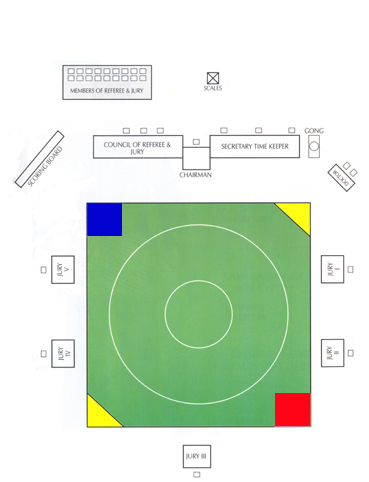
\includegraphics[width=0.5\textwidth]{images/competition_arena}
    \caption{Competition Arena}
 \end{figure}



    \begin{legal}
    \item For TANDING (Sparring Match) category, the specification should be as follows:
        \begin{legal}
        \item The competition arena: The area of the arena is a square with measurement of 10m x 10m. Inside the arena is a circle-shaped match ground of 8m diameter.
        \item The border between arena and match ground is marked with white line of ±5cm wide, drawn inwards.
        \item In the centre of the match ground a circle of 3m-diameter is drawn. The circles borderline is white and ± 5cm wide. This circles serves as a separating line at the start of a match.
        \item The Pesilat (contestants) corners are the arena squares corners diagonally facing each other and separated by the match ground; these corners consists of:
            \begin{legal}
            \item The blue corner located at the far right side of the competitions table.
            \item The red corner located diagonally across the blue corner.
            \item The yellow corners i.e. the two other corners, as neutral corners.
            \end{legal}
        \end{legal}
    \item For TUNGGAL (Solo Performance), GANDA (Choreographed Pair Performance) and REGU (Synchronized Team Performance) categories, the following specification is applied: The performance arena of the three categories is an area with a measurement of 10m x 10m.
    \end{legal}
\item The Arena Equipment: \\

The arena equipments which must be provided by the Organizing Committee consists of:

    \begin{legal}
    \item Competition tables and chairs
    \item Referee-Jurys tables and chairs
    \item Competition forms and stationeries
    \item Competition stopwatch, a gong (or any similar instruments) and a bell
    \item A Bout light or any other signalling instrument, to determine a round
    \item Red, blue and yellow signal lights to give signal when needed during the course of a competition
    \item A red and blue flag with a pole, each measuring 30cm x 30cm for the Jury of Tanding (Sparring Match) and another yellow flag with same measurements for the Timekeeper
    \item An information board displaying the duration time of Pesilats (contestants) performance in Tunggal, Ganda and Regu categories
    \item Weapon stand
    \item Scoring board
    \item Weighing scales
    \item Sound system
    \item Bucket, a mop, and floor mat
    \item Audio-visual recording instruments and the operator (this instrument is not a legitimate evidence for decision of the winner of a competition)
    \item Signage for Competition Chairman, Council of Referee-Jury, Secretary of Competition, Time Keeper, Doctors of Competition, Jury with sequence accordingly (1 to 5). If needed, the translation/local terms can be written underneath of each title
    \item   Other equipment whenever deemed necessary. For example, in a certain condition where the audience are too noisy resulting in the contestants inability to hear referees voice clearly, the referee may use a wireless microphone
    \end{legal}
\end{legal}

    \begin{figure}[t!]
    \centering
    \subfigure[Signal Lights (left), Round Lights (right)]{\label{fig:lights}
        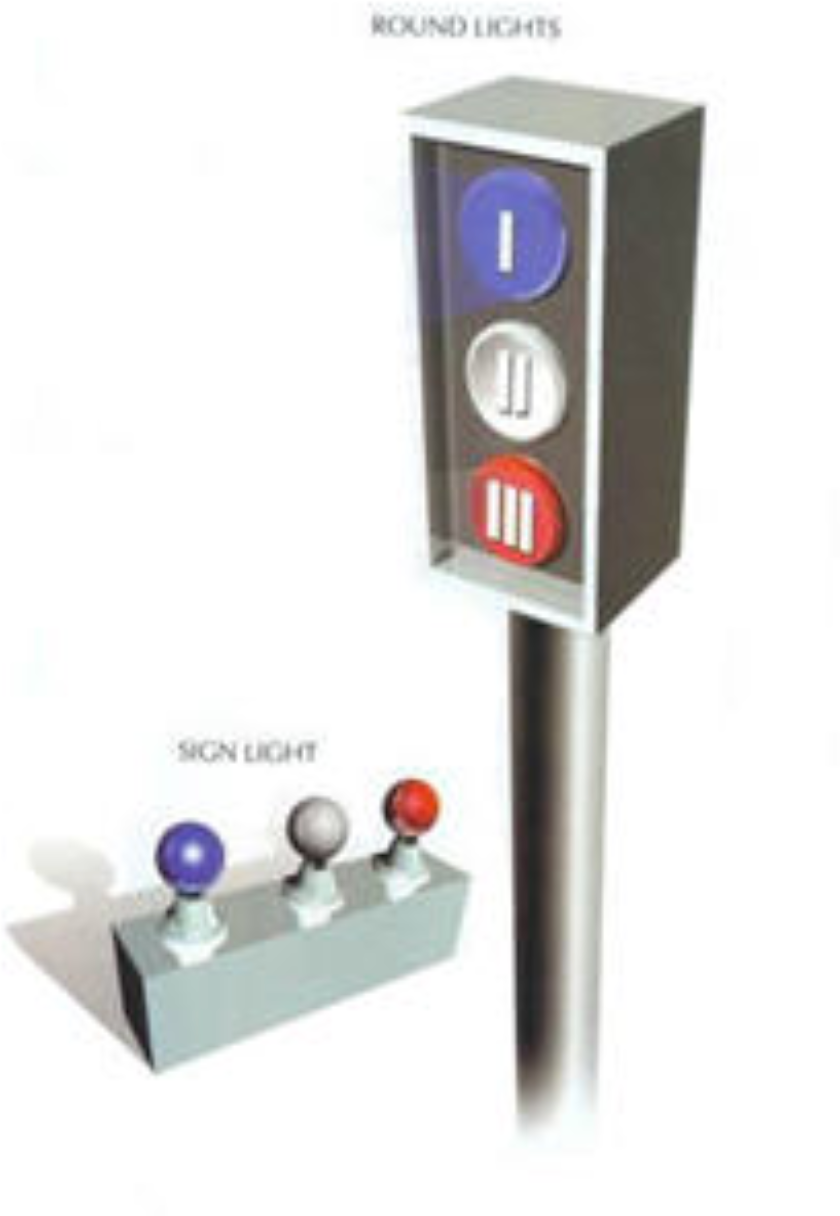
\includegraphics[height=2.2in]{images/round_lights}
    }
    ~
    \subfigure[Weapon Stands and Gong]{\label{fig:gong}
        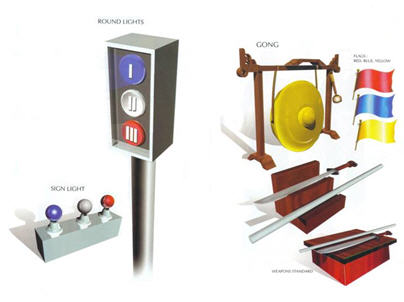
\includegraphics[height=2.2in]{images/gong}
    }
    \\
    \subfigure[Sound System]{\label{fig:sound_system}
        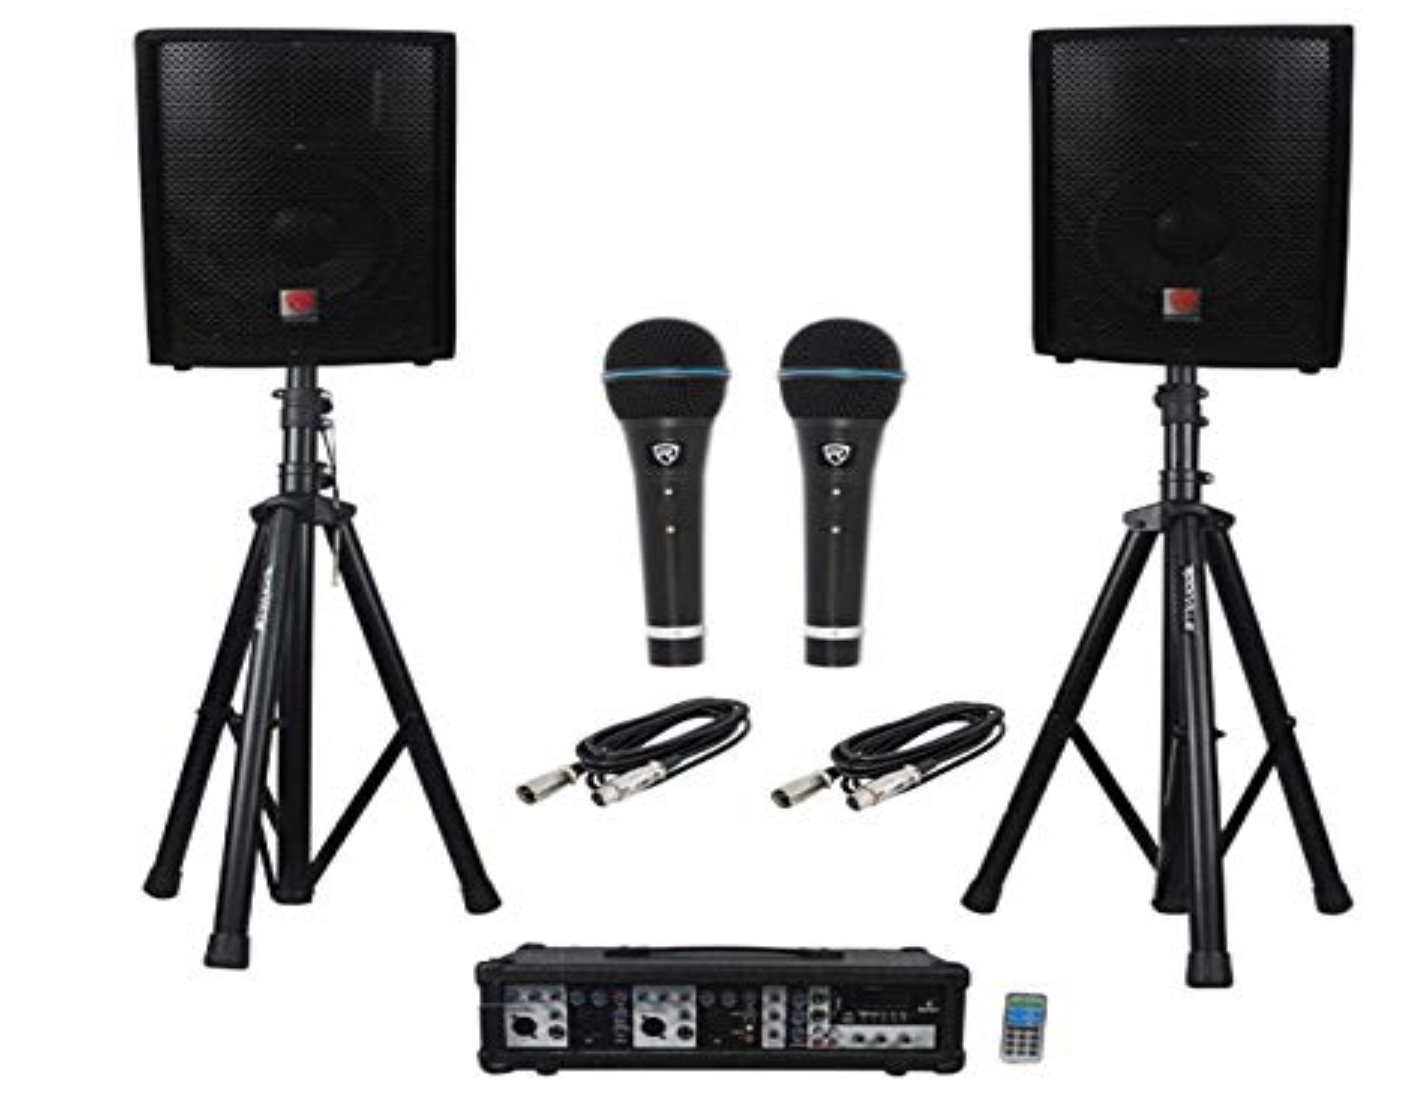
\includegraphics[height=2.2in]{images/sound_system}
    }
    ~
    \subfigure[Weigh-in Scale]{\label{fig:scale}
        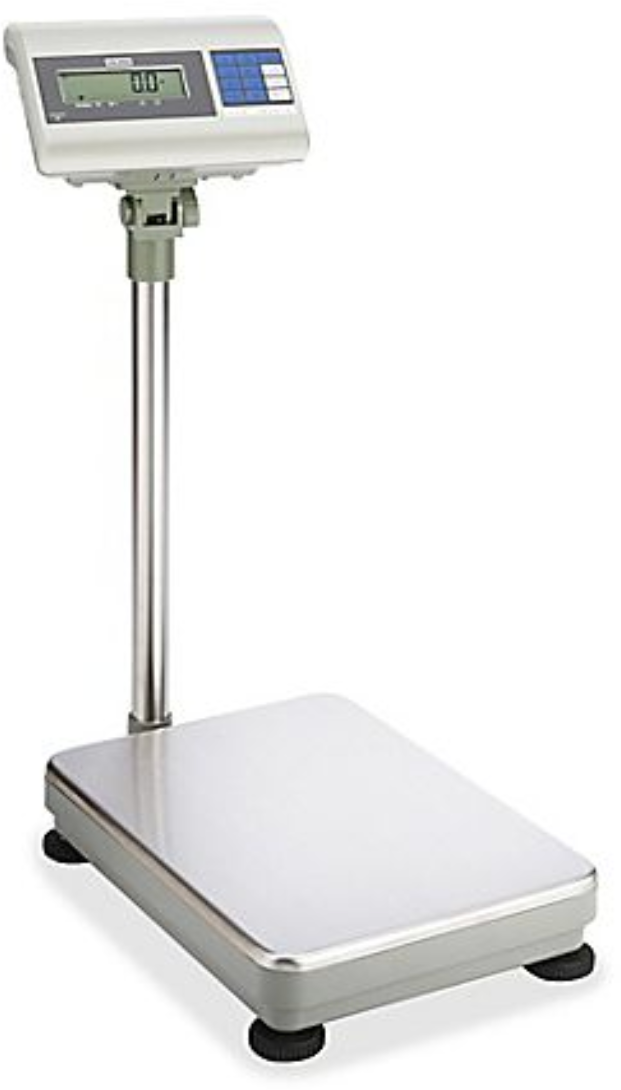
\includegraphics[height=2.2in]{images/scale}
    }
    \caption{Example Competition Equipment}
    \end{figure}
